\documentclass[english]{article}

\usepackage[latin9]{inputenc}
\usepackage[letterpaper]{geometry}
\geometry{verbose,tmargin=1in,bmargin=1in,lmargin=1in,rmargin=1in}
\usepackage{amsmath}
\usepackage{amssymb}
\usepackage{graphicx}

\newcommand{\grav}{\overrightarrow{g}}
\newcommand{\rotvec}{\overrightarrow{\theta}}

\title{ESE 650, Learning in Robotics, Spring 2016: Project2 \\
Yu-Cheng Lin}
\date{}

\begin{document}
\maketitle
\section*{Introduction}
This document describes my approaches to project 2: attitude estimation with accelerometer and gyroscope with Kalman filter. In all the plots of this document, red lines are always ground truth and blue lines are measured/estimated.
\section*{Calibration and obtaining ground truth}
Before calibration, I must obtain ground truth from the vicon data. The orientation was easy to recover since the vicon data conveniently provided rotation matrices. Note that the rotation matrices actually describes the rotation from the body frame to inertial frame. Therefore, I must rotate the gravity vector $[0 0 9.81]^T$ with the transpose of the given vicon data.
\[\overrightarrow{g_b} = R_{vicon}^T\overrightarrow{g_w} \]
where subscript w denotes world frame and b denotes body frame.\\
The angular velocity can be obtained by the numerical derivative of the orientation. However, I should not directly take the numerical derivative of a rotation matrix. Instead, I can describe a change in rotation $R_e$ so that the rotation at time step t $R_t$ can be followed by $R_e$ to obtain the rotation at time step t+1.
\[ R_tR_e = R_{t+1} \]
\[R_e = R_t^TR_{t+1} \]
Then, I can take this rotation $R_e$ and convert it to a rotation vector $\overrightarrow{\theta}$ such that $e^{\overrightarrow{\theta}} = R_e$. Take $\overrightarrow{\theta}$ and then divide by the elapsed time. I can get an estimate of the angular velocity. However, such reading is very noisy. To compensate for the noise, I ran the numerical derivative through a 6th order Butterworth filter to obtain smooth results.\\
The calibration for the sensors were done by inspection instead of linear regression. This works better because matching time stamps of vicon and the Imu is difficult (some interpolation will be needed), and linear regression is suceptable to noise. Perhaps a L-2 penalized linear regression with the values by inspection as prior can work very well, but it is not the focus of the project. Following plots are the results I obtained from training set 1.
\\\\
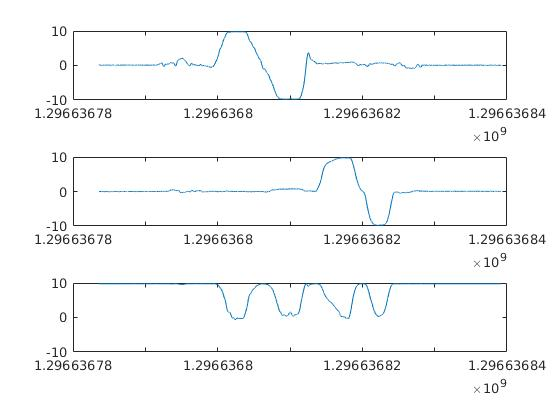
\includegraphics[scale=0.7]{vicon_g.jpg}\\
Expected gravity measurement given vicon data\\



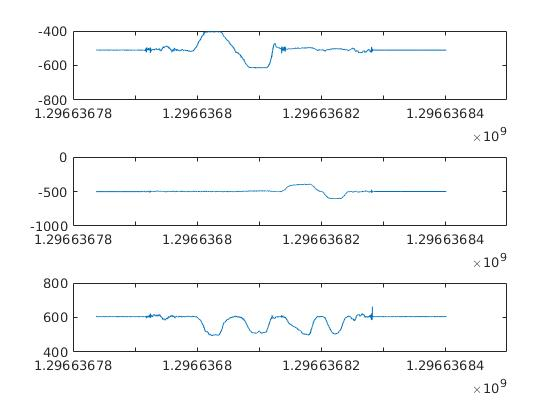
\includegraphics[scale=0.7]{imu_g.jpg}\\
measured gravity by IMU\\



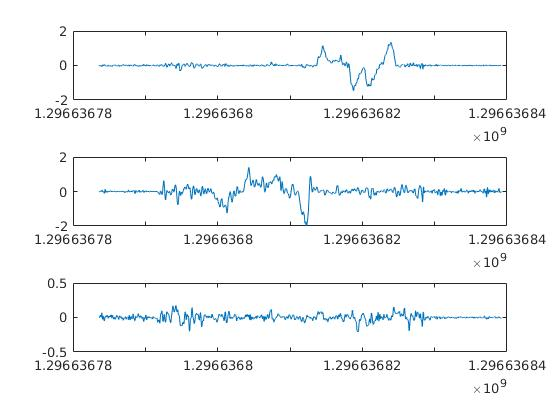
\includegraphics[scale=0.7]{vicon_omega.jpg}\\
Expected angular velocity measurement given vicon data\\



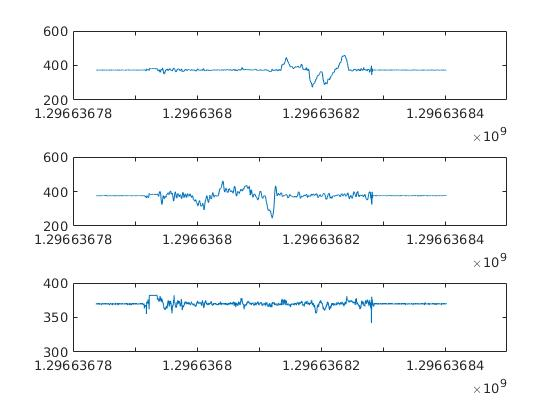
\includegraphics[scale=0.7]{imu_omega.jpg}\\
measured angular velocity by IMU\\


\section*{Obtaining Orientation with accelerometer}
It is mathematically impossible to obtain the full orientation with only one vector measurement. However, from this vector measurement, I can deduct two degrees of freedom in a rotatoin. Let's work under the framework of euler angles to get more intuition.\\
First, given a normalized gravity vector $\grav$ in the world frame with direction in $[0 0 1]^T$. and a rotation matrix $R$ from body frame to world frame. We can see that $R^T\grav$ picks out the third row of the rotation matrix $R$ and set them equal to the measured gravity.
\[
R_3 = \begin{bmatrix} g_x & g_y & g_z \end{bmatrix}
\]
Now, let's write $R$ in terms of euler angle with convention ZYX. 
\[R_3 = \grav^T = \begin{bmatrix}
\sin{\theta} & \cos{\theta}\sin{\phi} & \cos{\theta}\cos{\phi}
\end{bmatrix} \]
Here, we have two equations and two unknowns. Note that the gravity vector only gives me two degrees of freedom because it describes a direction (The vector has unit norm). The accleration alone does not give me any information about the Yaw.\\\\

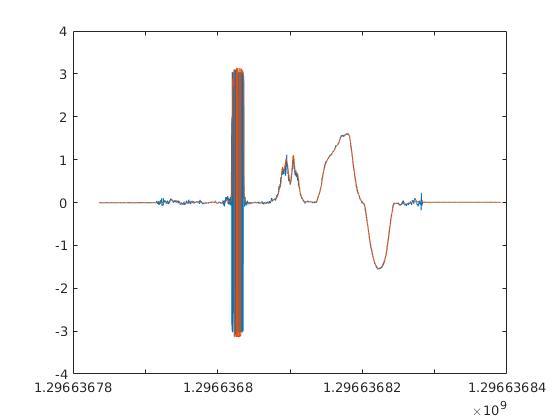
\includegraphics[scale = 0.7]{roll_acc.jpg}\\
measured roll angle by accelerometer\\
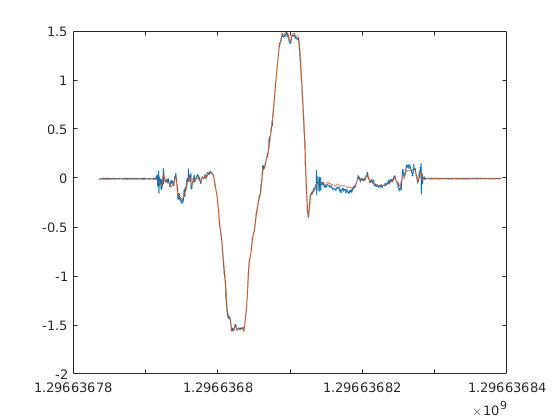
\includegraphics[scale = 0.7]{pitch_acc.jpg}\\
measured pitch angle by accelerometer\\

\section*{Obtaining Orientation with gyroscope}
The gyroscope can be numerically integrated to get the change in orientation. We can write the change of rotation as $\omega \Delta t$ so it's a rotation vector $\rotvec$. We can take the exponential of the anti-symmetric matrix form of this vector to obtain a differentail rotation matrix $\Delta R$. Post multiply this matrix to the current rotation matrix will give me the new rotation matrix.However, without knowledge of initial condition, this method can be very unreliable. For the puposes of this project, I will assume that the initial condition is at $R=I$.\\\\

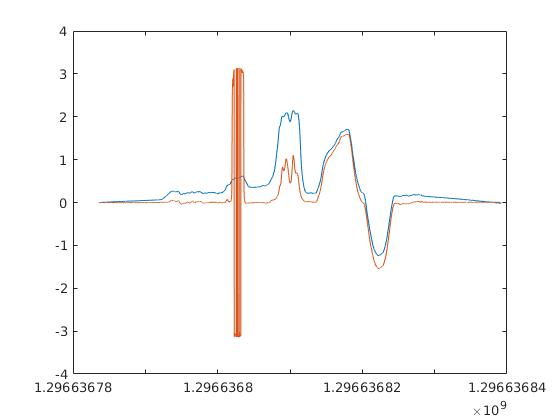
\includegraphics[scale = 0.7]{yaw_gyro.jpg}\\
measured roll angle by gyroscope\\
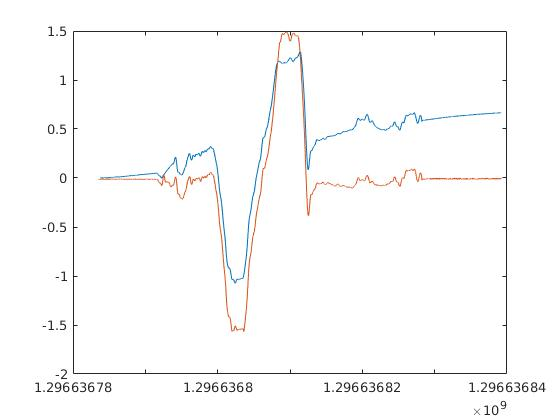
\includegraphics[scale = 0.7]{pitch_gyro.jpg}\\
measured pitch angle by gyroscope\\
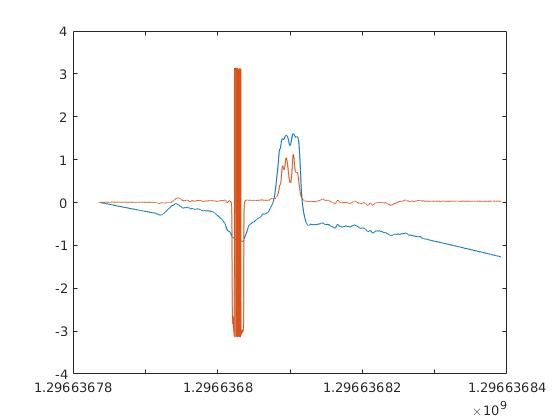
\includegraphics[scale = 0.7]{roll_gryo.jpg}\\
measured yaw angle by gyroscope\\

\section*{Unscented Kalman Filter}
From the two plots above, it is clear that we have to somehow merge the data from the two sensors to obtain a better estimate. The accelerometer gives us very good orientation information except that the yaw is missing. The gyroscope can estimate all three angles, but it needs a known initial condition. In addition, drift of bias is a big problem for the gyroscope.\\
Some kind of probalistic sensor fusion should be employed for this attitude estimation problem. Given the nonlinear nature of rotation, Unscented Kalman filter naturally suits this attitude estimation problem very well because of its ability to do nonlinear prediction and measurement. I followed the Kraft paper mainly but added in some small twists to improve my results.
\subsection*{Setup}
As illustrated earlier in this report, the gyroscope is unreliable if my calibration of the bias is off or if the bias drifts. To compensate for this, on top of the 7 states from the Krafts paper, I added three more states $[b_x, b_y, b_z]$ to account for the bias in the gyroscope. This modifies my measurement model
\[H(\omega^-, b^-) = \omega_{ADC}^-\]
where
\[H(\omega^-, b^-) = K_{\omega}*\omega^- + b^-\]
Although there are changes to the process model and the covariance matrices. They are just dimension changes. Thus, I will skip the discussion of these components.
\subsection*{Tuning}
Since the bias terms couples extra uncertainties to the angular velocity, blindly tuning R actually works better than measuring the covariance in the sensors. The rules of thumb is that since the data is fairly noisy, we would prefer very low covariance for the Q matrix to dampen the estimates.
\subsection*{Hacks}
Sometimes, undesired acceleration messes up the reading of the accelerometer. This can be detected by calculating the norm of the measured gravity. If the norm is out of a certain range, I will not take in the measurement at that time step and just use the dynamic model. However, the The a priori covariance $P^-$ grows very fast because of the nonlinear mapping of the sigma points. If there are many consecutive points that have bad readings, $P^-$ can grow too fast and make the Kalman filter unstable. In such cases, a simple hack is to return $P_{k-1}$, the covariance of the last step instead of the projected covariance. It's not mathematically correct, but it works reasonably well for this project.
\subsection*{Training Set Results}
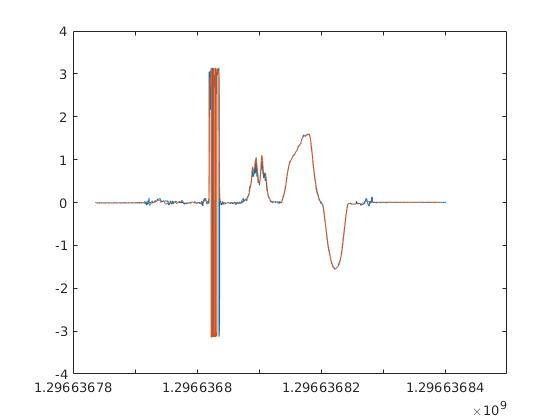
\includegraphics[scale = 0.7]{roll_kalman1.jpg}\\
roll angle of dataset1 estimated by my UKF\\
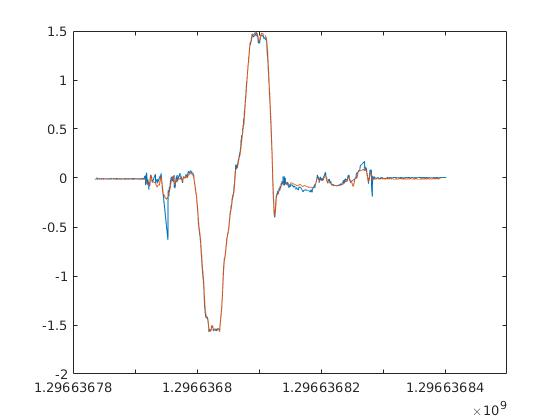
\includegraphics[scale = 0.7]{pitch_kalman1.jpg}\\
pitch angle of dataset1 estimated by my UKF\\
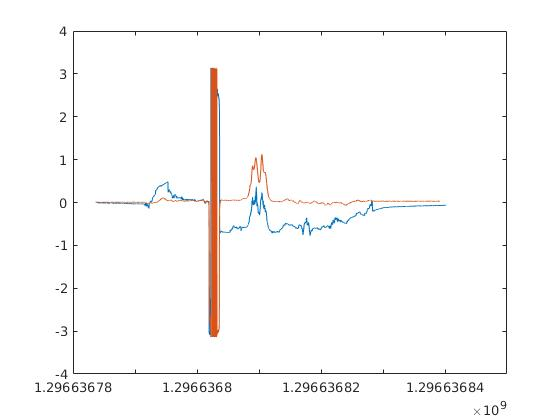
\includegraphics[scale = 0.7]{yaw_kalman1.jpg}\\
yaw angle of dataset1 estimated by my UKF\\

\end{document}
